for AB:-
\begin{align}
	\vec{m} &= \vec{B}-\vec{A}\\
         &= \myvec{-4-1\\6+1}\\
         &= \myvec{-5\\7}
\end{align}
we have to find $\vec{n}$,
\begin{align}
        \vec{n} &= \myvec{0&1\\-1&0}\vec{m}\\
                &= \myvec{0&1\\-1&0}\myvec{-5\\7}\\
                &= \myvec{7\\5}
\end{align}
\begin{figure}
\centering
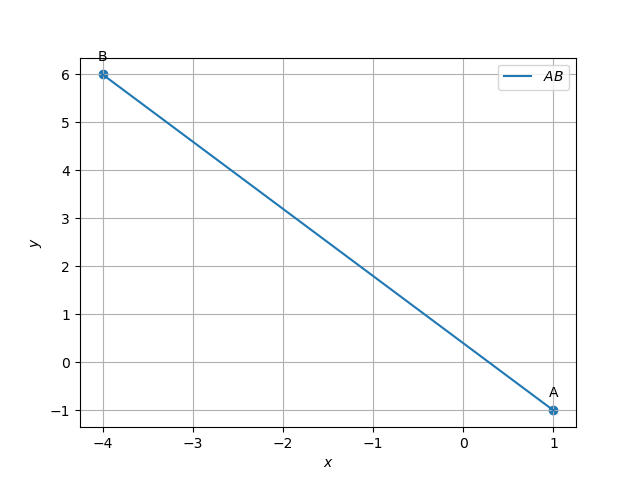
\includegraphics[width=\columnwidth]{solutions/1/1/5a/figs/figure1.png}
\caption{Line AB}
\label{fig:line AB}	
\end{figure}
normal form of equation of line AB:
\begin{align}
                \vec{n}^{\top}(\vec{x} - \vec{A}) &= 0\\     
       \implies \vec{n}^{\top}\vec{x} &= \vec{n}^{\top}\vec{A}\\ 
       \implies \vec{n}^{\top}\vec{x} &= \myvec{7&5}\myvec{1\\-1}\\    
       \implies\myvec{7&5}\vec{x} &= 2
\end{align}
